\newcommand{\dagmcModel}[2] {
  \null %emptyline
  \textbf{\uppercase{#1}} 
  \begin{adjustwidth}{2.5em}{0pt}
    #2
  \end{adjustwidth}
  \null
}

\chapter{Introduction}\label{ch:introduction}

Methods for modeling radiation transport determine particle flux, or derived
quantities, across space, angle, energy and time. The combination of the space,
angle, energy, and time domains is known as \textit{phase space}. The behavior
of these particles is described by the linear Boltzmann transport
equation \cite{Ulam_1949}. Deterministic solve this transport equation by discrectizing
the phase space of the problem, but time and memory constraints often limit the
resolution of phase space in practical problems.

The Monte Carlo approach to modeling Radiation transport simulates the
interaction of individual particles across the phase
space \cite{Lewis_1993}. This method was developed at Los Alamos National
Laboratory (LANL) during World War II by Fermi, von Neumann, Ulam, Metropolis,
and Richtmyer \cite{LANL_1987}. It uses a random walk process to solve the
transport equation. Pseudo-random numbers are used to sample probability
distribution functions representing properties of the virtual medium and in turn
determine the particle interaction outcomes. This stochastic approach requires
the simulation of many particles to reduce the statistical uncertainty of the
solution, where the uncertainty is inversely proportional to the square root of
the number of particles simulated. As the number of simulated particles
approaches infinity, tallied quantities approach the value of the continuous
solution.

The pros and cons of the two approaches complement each other. While
deterministic approaches inherently calculate a solution over the entire problem
domain, they take on additional error by discretizing phase space. In contrast,
Monte Carlo methods only incur error associated with input parameters such as
cross sections or geometry specifications, but it is challenging to achieve a
global solution with constant statistical error using this
approach. Computationally, deterministic methods typically suffer memory and
runtime costs that scale with the resolution of the discretized phase
space. Monte Carlo methods are typically limited by the runtime needed to
achieve satisfactory uncertainty in a region of interest.


\section{Monte Carlo Geometry}


Historically, Monte Carlo codes Constructive Solid Geometry (CSG) as their
\textit{native} geometry representation. CSG representations represent 3D
regions of virtual space using Boolean combinations of half spaces defined by
quadratic surfaces.To define the geometry, the surface definitions and the
Boolean combinations used to represent 3D regions (also referred to as cells or
volumes) are entered into a text file. This format for geometry is robust once
defined properly, but is limited in representation compared to more modern
geometric modeling tools such like Computer-Aided Design (CAD).

CAD allows for increased accuracy in model representation and better human
efficiency. CAD is able to represent higher-order surfaces and provides access
to models used for analysis in other engineering domains. These shared models
allow for a common problem domain in coupled simulation. CAD systems also provides a
rich set of tools for model generation, topological representation, and design
iteration. In highly complex and well-developed models, all of these tools are
more intuitive and efficient for human use over alteration of native text-based
formats. Many tools exist for converting native CSG models to and from CAD
systems, and a few have the capability to perform simulations directly on CAD
geometries.

The Direct Accelerated Geometry Monte Carlo (DAGMC) \cite{Tautges_2009} is one
of several software packages which enables Monte Carlo simulations on CAD-based
geometries. DAGMC's design allows it to serve as a particle
tracking and geometry kernel for a variety of Monte Carlo codes all of which are
listed in Table \ref{tab:dagmc_implementations}.

Specifically, it has been successfully integrated with MCNP, FLUKA, and Geant4
to date \cite{LANL_MCNP5_VOLIII, Bohlen_2014, GEANT4_2003}.

\begin{table}[H]
  \centering
  \begin{tabular}{c c}
    \hline
    Monte Carlo Code & DAGMC Implementation \\
    \hline
    MCNP5            & DAG-MCNP5            \\
    MCNP6            & DAG-MCNP6            \\
    Fluka            & FluDAG               \\
    Tripoli4         & DAG-Tripoli4         \\
    Geant4           & DagSolid             \\
    Shift            & DAG-Shift            \\
    \hline
  \end{tabular}
  \caption{A list of Monte Carlo codes and the names of their corresponding DAGMC implementations.}
  \label{tab:dagmc_implementations}
\end{table}

\section{Statement of Problem}\label{sec:problem-statement}

While the use of CAD geometries brings the benefits outlined above, it also adds
complexity to particle tracking during Monte Carlo simulations. Particle
crossings with higher-order surfaces are difficult and sometimes impossible to
compute. To address this problem, the analytic CAD surfaces are
discretized into a triangle mesh. This has the effect of generalizing surface crossings to
intersections with a set of planar surfaces if one were to define the same
surface or volume using CSG. In this way, robust surface crossings for highly
accurate representations of higher order surfaces and complex geometries are
achieved. However, a large number of triangles are needed to maintain an
accurate representation of surfaces throughout the model. As a result, the
costly search for surface crossings causes simulations on CAD-based geometries
to take much longer than native CSG models.

The intersection of a particle and trajectory with a triangulated surface is a
well-researched problem in the area of ray tracing. In this field, geometries
are also triangulated for visualization and rendering purposes. DAGMC currently
employs some techniques from this field to accelerate geometric queries, but it
remains much slower than native geometry implementations in CSG. DAGMC's
simulations are anywhere from 2.5 to 10 times longer than those of their native
counterparts.

\subsection{Performance Results}%%Status:Done%%

Table \ref{dag-mcnp-benchmarks} represents a comparison of several
representative MCNP problems when run the native geometry representations and
DAGMC coupled with MCNP, or DAG-MCNP.For smaller problems with simple geometries
and relatively low numbers of histories required to reach an acceptably low
level of statisitcal uncertainty, this might not pose as much of a problem to
users. As problem geometries become more complicated and the number of histories
becomes larger however, the discrepancy in computing time becomes of high
importance when run times extend to days or weeks longer than they would using
the native MCNP CSG geometry representation. These models include the Frascati
Neutron Generator (FNG), the Advanced Test Reactor (ATR), and the University of
Wisconsin Nuclear Reactor (UWNR).

\begin{table}[H]
  \centering
  \begin{tabular}{l c c c}
    \toprule
    Model & Native ctme (min) & DAG-MCNP ctme (min) & Ratio (Native/DAGMC) \\
    \hline
    FNG   & 5871.92           & 22769.33            & 3.9                  \\
    ATR   & 901.68            & 8627.80             & 9.6                  \\
    UWNR  & 8767.29           & 69429.60            & 7.9                  \\
    \hline
  \end{tabular}
  \caption{Table comparing the performance of DAG-MCNP to native MCNP for the same modules after translation to a CAD-based surface mesh.}
  \label{dag-mcnp-benchmarks}  
\end{table}

As a part of this study, these runs were repeated using the profiling tool,
Callgrind, within KCachegrind to determine where is being spent in both the
DAG-MCNP and native MCNP runs. Because the geometry representation and query
system is the only difference between the two models, it is expected that the
time is being spent there, but it is practical to confirm this and useful to
know more specifically where in the query system this is occuring. All
callgraphs are displayed with the MCNP \textit{history\_} subroutine at the
top. It is inside this subroutine that MCNP calls upon DAGMC to fulfill
geometric queries about the model. It should also be noted that for these
profiling runs the fcad file produced by a previous DAGMC run was used. DAGMC
produces this file after completing the BVH build for a given geometry. Using
this file keeps the profiling information from being obfuscated by the building
process of the BVH in MOAB and allows DAG-MCNP to move straight to particle
transport after loading the geometry and BVH from the fcad file.

In Figure \ref{dagmc-fng-coarse} a callgraph for a profiling run of FNG for 1e7
histories is provided. In this callgraph it is shown that the time spent in
transport is dominated by MOAB's ray tracing process used by DAGMC to track
particles as they move through the geometry. About 60\% of the runtime is spent
in DAGMC's \textit{ray\_fire} while in native MCNP the relative time spent on
this process is reduced to ~5\% with the majority of the time spent in
calculating cross sections under the textit{acetot\_} subroutine.

\begin{figure}[H]
  \centering
  \caption{Callgraph of DAG-MCNP FNG run for 1e7 histories. (Processes taking
    $<$10\% of the runtime are filtered out in order to simplify the callgraph.)}
  \label{dagmc-fng-coarse}
  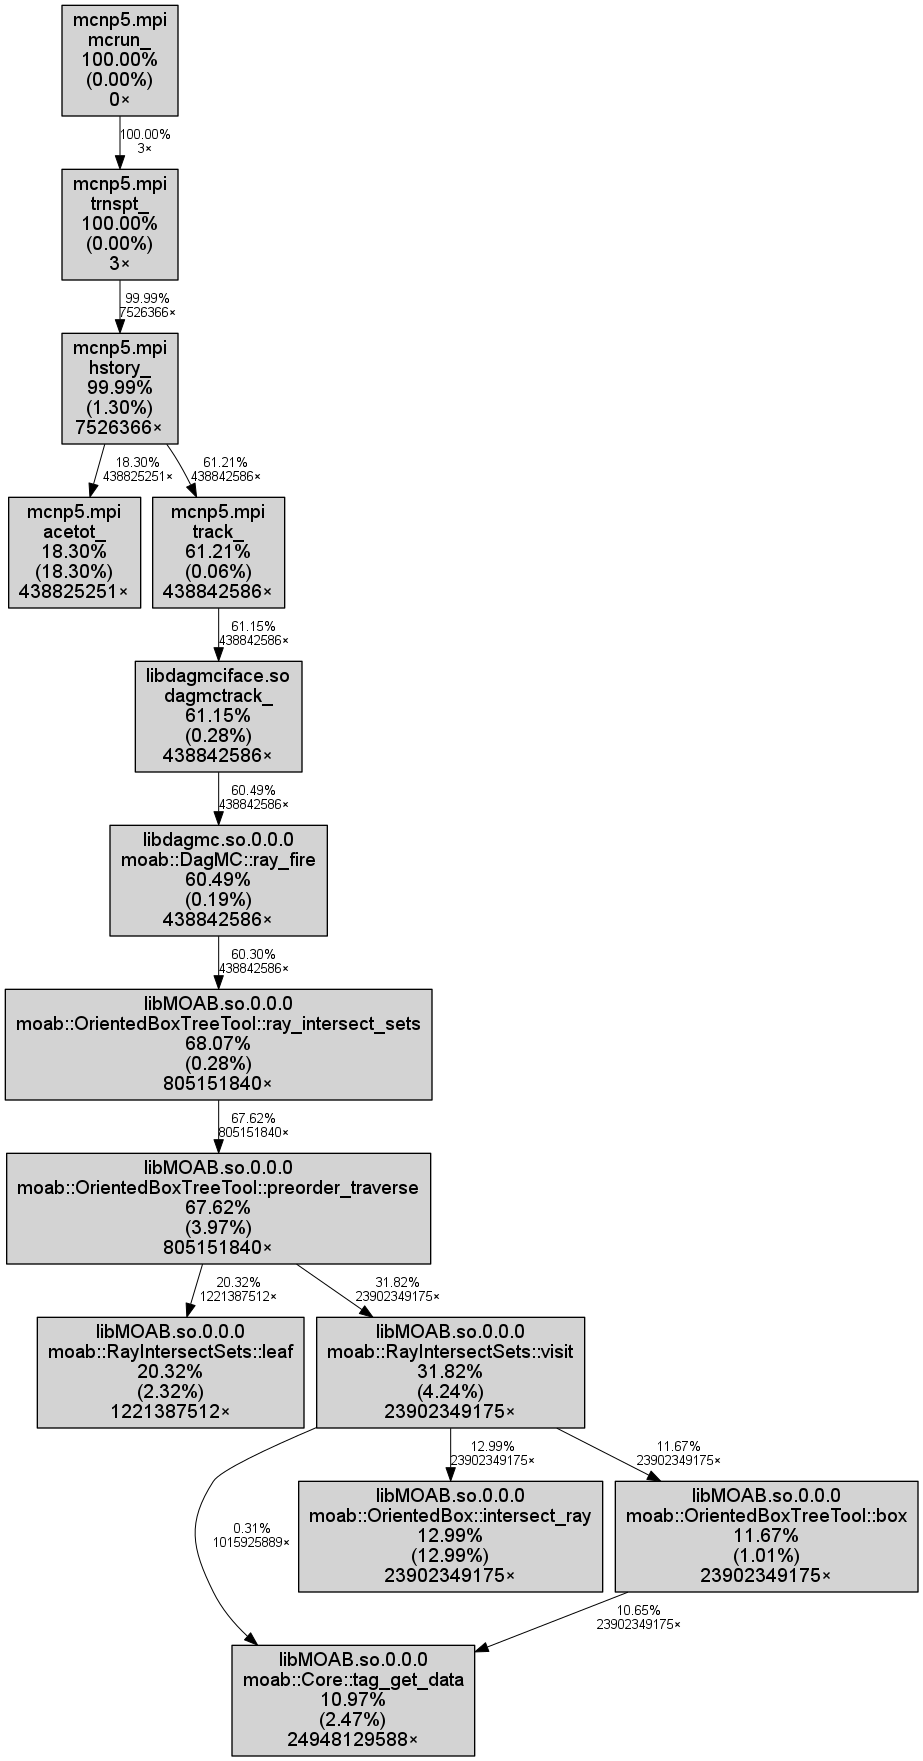
\includegraphics[scale=0.3]{dagmc_fng_cg_coarse.png}
\end{figure}

\begin{figure}[H]
  \centering
  \caption{Callgraph of native MCNP FNG run for 1E7 histories. (Processes taking
    $<$10\% of the runtime are filtered out in order to simplify the call
    graph.)}
  \label{mcnp-fng-coarse}
  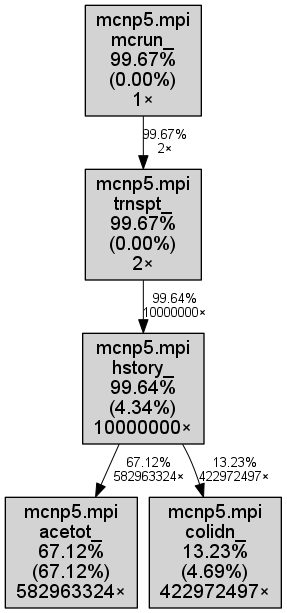
\includegraphics[scale=0.3]{native_fng_cg_coarse.png}
\end{figure}


It should be noted that in this case a pre-built BVH was include in
the geometry file and read into place much more quickly than in a typical DAGMC
run. While this processes does contribute to additional DAGMC runtime, the
amount of time spent building these hierarchies is small relative to the time
spent in particle transport due to the high number of histories required for
good statistics in the Monte Carlo results.

The combination of the profiling results indicating how much time is spent in
tracking particles in DAGMC along with the difference in absolute run times
confirms that indeed the performance bottleneck of DAGMC lies in its ability to
quickly satisfy the geometric queries of the underlying Monte Carlo code it is
coupled to. Looking more closely at the underlying calls in DAGMC, one can see
that this time is collectively spent in the DAGMC \textit{ray\_fire} call with
the BVH traversal lying below this along with many underlying MOAB
database-related calls. This indicates that this time is spent even more
specifically in traversing MOAB's OBB BVH via the database-oriented methods
available in DAGMC.

\section{Statement of Thesis}

The purpose of this dissertation is to establish work that improves the
performance of CAD-based Monte Carlo radiation transport in a manner that is
widely accessible to analysts. The result is a compilation of adaptive data
structure construction, data structure redesign, and alternative methods to
reduce simulation times in DAGMC.

%% Developments in CPU architecture have prompted the redesign of ray tracing data
%% structures and enabled enhanced performance of these queries. This is
%% exemplified in the Embree project developed by Intel \cite{Wald_2014} which has
%% been applied to CAD-based Monte Carlo analysis. This project


